\documentclass[11pt,oneside,letterpaper]{article}

% graphicx package, useful for including eps and pdf graphics
\usepackage{graphicx}
\usepackage{grffile}
%\DeclareGraphicsExtensions{.pdf,.png,.jpg}

% basic packages
\usepackage{color} 
\usepackage{parskip}
\usepackage{float}
\usepackage{microtype}
\usepackage{url}

% reference figures across documents
\usepackage{xr}
%\externaldocument{EBOV_phylogeography_supp}

\usepackage{longtable}

% text layout
\usepackage{geometry}
\geometry{textwidth=15cm} % 15.25cm for single-space, 16.25cm for double-space
\geometry{textheight=22cm} % 22cm for single-space, 22.5cm for double-space

% helps to keep figures from being orphaned on a page by themselves
\renewcommand{\topfraction}{0.85}
\renewcommand{\textfraction}{0.1}

% bold the 'Figure #' in the caption and separate it with a period
% Captions will be left justified
\usepackage[labelfont=bf,labelsep=period,font=small]{caption}

% review layout with double-spacing
%\usepackage{setspace} 
%\doublespacing
%\captionsetup{labelfont=bf,labelsep=period,font=doublespacing}

% cite package, to clean up citations in the main text. Do not remove.
%\usepackage{cite}
\usepackage{natbib}
%\renewcommand\citepleft{(}
%\renewcommand\citepright{)}
%\renewcommand\citepform[1]{\textsl{#1}}

\usepackage{amsmath}

% Remove brackets from numbering in list of References
%\renewcommand\refname{\large References}
%\makeatletter
%\renewcommand{\@biblabel}[1]{\quad#1.}
%\makeatother

\usepackage{authblk}
\renewcommand\Authands{ \& }
\renewcommand\Authfont{\normalsize \bf}
\renewcommand\Affilfont{\small \normalfont}
\makeatletter
\renewcommand\AB@affilsepx{, \protect\Affilfont}
\makeatother

% comments
\usepackage{ulem}
\definecolor{purple}{rgb}{0.459,0.109,0.538}
\def\tb#1#2{\sout{#1} \textcolor{purple}{#2}} 
\def\tbc#1{\textcolor{purple}{[#1]}}

%GLM-CTMC
\newcommand{\rateMatrix}{\ensuremath{\boldsymbol{\Lambda_{t}}}}
\newcommand{\rateMatrixElement}{\ensuremath{\Lambda_{ij}}}
\newcommand{\coefficient}{\ensuremath{\beta}}
\newcommand{\increment}{\ensuremath{\beta}}
\newcommand{\coefficientSpace}{\ensuremath{\beta} }
\newcommand{\indicator}{\ensuremath{\delta}}
\newcommand{\predictor}{x}
\newcommand{\idxPredictor}{p}
\newcommand{\transpose}{^{'}}
\newcommand{\numPredictors}{P}
\newcommand{\before}{P}
\newcommand{\timeIndicator}{\phi}
\newcommand{\indicatorFunction}[1]{\ensuremath{1_{ #1 }}}
\newcommand{\rateMatrixMAS}{\boldsymbol{\Lambda}}
\newcommand{\rateMatrixElementMAS}{\Lambda_{ijt}}
\newcommand{\predictorLabel}[1]{_{\mbox{\tiny #1}}}
\newcommand{\randomEffect}{\epsilon}
\newcommand{\numLocations}{K}
\newcommand{\markA}{\text{\tiny B}}
\newcommand{\markB}{\text{\tiny A}}


\newcommand{\incIndicator}{\delta}


%%% TITLE %%%
\title{\vspace{1.0cm} \LARGE \bf Supplementary Document}

\date{\today}

\begin{document}
\maketitle

\begin{abstract}


\end{abstract}

\pagebreak

\section*{Methods}

\subsection*{Sequence data}

The data set consists of 1610 full Ebola virus (EBOV) genomes sampled between 17 March 2014 and 24 October 2015. 
The number of sequences and the proportion of cases sequenced varies with country; our data set contains 209 sequences from Liberia (3.8\% of known and suspected cases), 982 from Sierra Leone (8.0\%) and 368 from Guinea (9.2\%) (Table~\ref{caseTable}).
Most (1100) genomes are of high quality, with ambiguous sites and gaps comprising less than 1\% of total alignment length, followed by sequences with between 1\% and 2\% of sites comprised of ambiguous bases or gaps (266), 98 sequences with 2-5\%, 120 sequences with 5-10\% and 26 sequences with more than 10\% of sites that are ambiguous or are gaps.
Sequences known to be associated with sexual transmission or latent infections were excluded, as these viruses often exhibit anomalous molecular clock signals, although it is difficult to ascertain whether sequences from such cases were not included in the final data set if they were collected at the height of the epidemic.
Sequences were aligned using MAFFT \citep{katoh_2002} and edited manually.
The alignment was partitioned into coding regions and non-coding intergenic regions and concatenated such that coding sequences are connected end to end, followed by intergenic regions separated from the coding sequences by a spacer of three N's.
The final alignment length was 18992 nucleotides.
 
\subsection*{Masking putative ADAR edited sites}

As noticed by \citet{tong_2015}, \citet{park_2015} and other studies, some EBOV isolates contain excessive numbers of T-to-C mutations within relatively short stretches of the genome. 
Interferon-inducible adenosine deaminases acting on RNA (ADAR) are known to induce adenosine to inosine hypermutations in double-stranded RNA \citep{bass_1988}.
ADARs have been suggested to act on RNAs from numerous groups of viruses \citep{gelinas_2011}. 
When negative sense single stranded RNA virus genomes are edited by ADARs, A-to-G hypermutations seem to preferentially occur on the negative strand, which results in U/T-to-C mutations on the positive strand \citep{cattaneo_1988,rueda_1994,carpenter_2009}. 
Multiple T-to-C mutations are introduced simultaneously via ADAR-mediated RNA editing which would interfere with molecular clock estimates and, by extension, the tree topology.
We thus designate four or more T-to-C mutations within 300 nucleotides of each other as a putative hypermutation tract, whenever there is evidence that all T-to-C mutations within such stretches were introduced at the same time, \textit{i.e.} every T-to-C mutation in a stretch occurred on a single branch.
We detect a total of 15 hypermutation patterns with up to 13 T-to-C mutations within 35 to 145 nucleotides.
Of the 15 hypermutation patterns we detect 11 are found in single genomes and four are shared across 67 strains.
Putative tracts of T-to-C hypermutation almost exclusively occur within non-coding intergenic regions, where their effects to viral fitness are presumably minimal. 
Hypermutation tracts are usually found in individual sequences, further supporting the hypothesis that they are deleterious to EBOV fitness. 
Nevertheless, some lineages that survive hypermutation are transmitted and are subsequently found in more than one isolate \citep{smits_2015}. 
In these cases we leave the first T-to-C mutation unmasked to provide phylogenetic information on the relatedness of these sequences.

\subsection*{Phylogenetic inference}
Molecular evolution was modelled according to a HKY$+\Gamma_{4}$ \citep{hky_1985,yang_1994} substitution model independently across four partitions (codon positions 1, 2, 3 and non-coding intergenic regions).
Evolutionary rates were modelled with branch-specific rates drawn from a relaxed molecular clock following a log-normal distribution \citep{drummond_2006} and site-specific rates scaled by relative rates in the four partitions.
A non-parametric coalescent `Skygrid' tree prior was employed for demographic inference \citep{gill_2012}.
The overall evolutionary rate was given an uninformative CTMC reference prior \citep{ferreira_2008}, while the rate multipliers for each partition were given an uninformative uniform prior over their bounds
All other priors used to infer the phylogenetic tree were left at their default values.

Two independent MCMC chains were run in BEAST 1.8.3 \citep{drummond_2012} for 100 million states, sampling every 10 000 states. 
The first 1000 samples in each chain were removed as burnin, and the remaining 18 000 samples combined between the two runs.
These 18 000 samples were used to estimate a maximum clade credibility tree and to estimate posterior densities for individual parameters.

\subsection*{Geographic history reconstruction}

The level of administrative division within each country was chosen so that population sizes between divisions are comparable. 
For each country the appropriate administrative divisions were: prefecture for Guinea (administrative subdivision level 2), county for Liberia (level 1) and district for Sierra Leone (level 2). 
We refer to them as locations (63 in total) and each sequence, where available, was assigned the location where the patient was recorded to have been infected as a discrete trait. 
When exact location was unknown, but other information, such as country, was available we inferred the sequence location as a latent variable with equal prior probability over all available locations within that country. 
In the absence of all geographic information we inferred both the country and the location of a sequence.

An asymmetric continuous-time Markov chain (CTMC) \citep{lemey_2009,edwards_2011} matrix was used to infer instantaneous transition rates between locations. 
Due to the complexity of the transition matrix a Bayesian stochastic search variable selection (BSSVS) procedure was used to select among all possible diffusion pathways \citep{lemey_2009}, with a Poisson prior on the number of non-zero entries in the migration matrix, with mean $\ln 2$ and offset = $K-1$, where $K$ is the number of locations.
This approach gives $0.5$ prior probability \textit{a priori} to the minimum number of transitions needed to keep the migration network connected.

We conditioned the phylogeographic analyses results for the genetic data to avoid the spatial information exerting an influence on the trees. \tbc{Will run test to check if this is an issue.}
This was done by drawing a sample of 1000 trees from the posterior set from the phylogenetic analysis and then allowing the phylogeographic analyses to switch between them with equal probability over the course of the MCMC.

To infer the spatial phylogenetic diffusion history between the $\numLocations = 63$ locations, we adopt a sparse generalised linear model (GLM) formulation of continuous-time Markov chain (CTMC) diffusion \citep{lemey_2014}.
This model parameterizes the instantaneous movement rate $\rateMatrixElement$ from location $i$ to location $j$ as a log-linear function of $\numPredictors$ potential predictors $\mathbf{X}_{ij} = \left( x_{ij1} , \ldots, x_{ij \numPredictors} \right)\transpose$ with unknown coefficients $\boldsymbol{\coefficient} = (\coefficient_1, \ldots, \coefficientSpace_{\numPredictors})\transpose$ and 
diagonal matrix $\boldsymbol{\incIndicator}$ with entries $\left( \incIndicator_1, \ldots, \incIndicator_{\numPredictors} \right)$.
These latter unknown indicators $\incIndicator_{\idxPredictor} \ \in \{0,1\}$ determine predictor $\idxPredictor$'s inclusion in or exclusion from the model.
We generalize this formulation here to include two-way random effects that allow for location origin- and destination-specific variability.  
Our two-way random effects GLM becomes
\begin{equation}
\begin{aligned}
\log \rateMatrixElement &= \mathbf{X}_{ij}\transpose \boldsymbol{\incIndicator} \boldsymbol{\beta}
+ \epsilon_i + \epsilon_j, \\
\epsilon_k &\sim \text{Normal}(0, \sigma^2) \text{ for } k = 1, \ldots, \numLocations, \text{ and} \\
\sigma^{2} &\sim \text{Inverse-Gamma}(0.001, 0.001),
\end{aligned}
\end{equation}
where 
$\boldsymbol{\epsilon} = \left( \epsilon_{1}, \ldots, \epsilon_{\numLocations} \right)$ are the location-specific effects.
These random effects account for unexplained variability in the diffusion process that may otherwise lead to spurious inclusion of predictors.

We follow \cite{lemey_2014} in specifying that \textit{a priori} all $\coefficient_{\idxPredictor}$ are independent and normally distributed with mean 0 and a relatively large variance of 4 and in assigning independent Bernoulli prior probability distributions on $\indicator_{\idxPredictor}$.
We use a small success probability on each predictor's inclusion that reflects a 50\% prior probability on no predictors being included. 
To draw posterior inference, we enjoy the success of \cite{lemey_2014} on integrating $\boldsymbol{\beta}$ and $\boldsymbol{\incIndicator}$, further employ a random-walk Metropolis transition kernel on $\boldsymbol{\epsilon}$ and to sample $\sigma^2$ directly from its full conditional distribution using Gibbs sampling.

For analyses that consider time-inhomogeneity in the diffusion process, we start by borrowing epoch modelling concepts from \cite{bielejec_epoch_2014}.
The epoch GLM parameterizes the instantaneous movement rate $\rateMatrixElementMAS$ from state $i$ to state $j$ within epoch $t$ as a log-linear function of $\numPredictors$ epoch-specific predictors $\mathbf{X}_{ijt} = \left( x_{ijt1} , \ldots, x_{ijt \numPredictors} \right)\transpose $ with constant-through-time, unknown coefficients $\boldsymbol{\coefficient}$. 
We generalize this model to incorporate time-varying contribution of the predictors through time-varying coefficients $\boldsymbol{\coefficient}(t)$ using
a series of change-point processes.  
Specifically, the time-varying epoch GLM models
\begin{equation}
\begin{aligned}
\log \rateMatrixElementMAS &= \mathbf{X}_{ijt}\transpose 
\boldsymbol{\beta} (t) \\
\boldsymbol{\beta} (t) &= 
\left[
\mathbf{I} - \boldsymbol{\timeIndicator}(t) \right] 
\boldsymbol{\coefficient}_{\markA} + 
\left[
\boldsymbol{\timeIndicator}(t) 
\right] \boldsymbol{\beta}_{\markB} ,
\end{aligned}
\end{equation}
%
where 
$\boldsymbol{\coefficient}_{\markA} = \left(\coefficient_{\markA1}, \ldots, \coefficient_{\markA\numPredictors} \right)\transpose$ are the unknown coefficients before the change-points,
$\boldsymbol{\coefficient}_{\markB} = \left(\coefficient_{\markB1}, \ldots, \coefficient_{\markB\numPredictors} \right)\transpose$ are 
the unknown coefficients after the change-points,
diagonal matrix $\boldsymbol{\timeIndicator}(t)$ has entries
$\left( \indicatorFunction{t > t_1}(t), \ldots, \indicatorFunction{t > t_{\numPredictors}}(t) \right)$,
$\indicatorFunction{(\cdot)}(t)$ is the indicator function and
$\mathbf{T} = (t_1, \ldots, t_{\numPredictors})$ are the unknown change-point times.
%, 
In this general form, the contribution of predictor $p$ before its change-point time $t_p$ is 
$\coefficient_{\markA p}$
and its contribution after is 
$\coefficient_{\markB p}$
for $p = 1,\ldots,\numPredictors$.  
Fixing $t_p$ to be less than the time of the first epoch or greater than the time of the last epoch results in a time-invariant coefficient for that predictor.

Similar to the constant-through-time GLM, we specify that \textit{a priori} all $\coefficient_{\markA p}$ and 
 $\coefficient_{\markB p}$
%$\increment_{p}$ 
are independent and normally distributed with mean 0 and a relatively large variance of 4.
When random, each $t_p$ is equally likely to lie before any epoch.
We employ random-walk Metropolis transition kernels on $\boldsymbol{\coefficient}_{\markA}$, 
$\boldsymbol{\coefficient}_{\markB}$
%$\boldsymbol{\increment}$ 
and $T$.
%
We perform the epoch GLM analysis including the five predictors that were supported in the time-homogeneous analysis:  distance (dis), a within country (wco) effect, a shared international border (sib) effect and origin and destination case counts.
We assume that origin and destination case count coefficients are time-invariant since their respective predictors already vary through time (by month), complicating model parameter identifiability.
Further, a preliminary study assumed that change-point times $t\predictorLabel{dis}$, $t\predictorLabel{wco}$ and $t\predictorLabel{sib}$ for the dis, wco and sib predictors were \textit{a priori} independent. 
Initial analysis indicated that $t\predictorLabel{sib}$ was difficult to estimate accurately, but its posterior mode was close to that of $t\predictorLabel{wco}$.
Therefore, we further assume $t\predictorLabel{sib} = t\predictorLabel{wco}$.

\subsection*{Case numbers}

Ebola virus disease (EVD) case numbers are reported by the WHO for every country division (district) at the appropriate administrative level, split by epidemiological week.
For every district and for each epidemiological week four numbers are reported: new cases in the patient and situation report databases as well as whether the new cases are confirmed or probable.
At the height of the epidemic many cases went unconfirmed, even though they were likely to have been genuine EVD.
As such, we treat probable EVD cases in WHO reports as confirmed and combine them with lab-confirmed EVD case numbers.
Following this we take the higher combined case number of situation report and patient databases.
The latest situation report in our data goes up to the epi week lasting from 8 to 14 February 2016, with all case numbers being downloaded on 22 February 2016.
There are apparent discrepancies between cumulative case numbers reported for each country over the entire epidemic and case numbers reported per administrative division over time, such that our estimate for the final size of the epidemic, based on case numbers over time reported by the WHO, is on the order of 22 000 confirmed and suspected cases of EVD compared to the official estimate of around 28 000 cases.
This probably arose because case numbers are easier to track at the country level, but become more difficult to narrow down to administrative subdivision level, especially over time.

%\subsection*{Predictors of viral spread}
%
%Generalized linear models (GLMs) were used to test the association between inter-location viral migration and these predictors. 
%GLM methods have been used in the past to identify intuitive factors behind geographic diffusion in well-studied viral migration systems and, for example, identified air traffic as a major contributor to the global dispersal of H3N2 subtype of influenza A virus \citep{lemey_2014}.
%We compiled a large set of potential predictors of EBOV spread in West Africa (Table~\ref{predictorTable}).

%\begin{figure}[H]
% \centering		
%	\includegraphics[width=0.85\textwidth]{figures/Fig 4. EBOV_1561_coefficients.pdf}
%	\caption{\textbf{Summary of general linear model results.}
%	Six predictors were found to be strongly correlated (Bayes factor$>$3) with geographic spread of EBOV. 
%	Blue bars one the right hand side indicate the proportion of time the given predictor matrix was included in the model over the course of MCMC.
%	Dashed lines show inclusion probability cut-offs where Bayes factor equals 3, 15 and 50.
%	Origin and destination location case counts, location pairs that are in different countries but share a border, locations within the same country and asymmetric flow of lineages from Liberia into Guinea were found to be positively correlated (in green) with the diffusion of EBOV lineages.
%	Great circle distances were found to be inversely (in red) correlated with EBOV migration.
%	Predictors that were not strongly supported are shown in grey.
%	}
%	\label{predictors}
%\end{figure}
%
%\begin{figure}[H]
% \centering		
%	\includegraphics[width=0.85\textwidth]{figures/Fig 5. epoch_dynamics.pdf}
%	\caption{\textbf{Summary of the epoch model.}
%	Epochs
%	}
%	\label{epochs}
%\end{figure}

\setcounter{figure}{0}
\setcounter{table}{0}
\setcounter{page}{1}
\renewcommand{\thefigure}{S\arabic{figure}}
\renewcommand{\thetable}{S\arabic{table}}
\renewcommand{\thepage}{S\arabic{page}}
  
\section*{Supporting Information}

%% Table of admin subdivisions, number of cases and number of samples?
\begin{longtable}{ | l | l | r | r | r | }
\caption{Number of cases and sampled sequences per location and country, where `Location' is standardised location name and `Sampling frequency' is sequences/cases $\times$ 100.}
\label{caseTable}\\
\hline
Country & Location & Sequences & Cases & Sampling freq.\\ 
\hline
GIN & Macenta & 40 & 784 & 5.10 \\
GIN & Conakry & 73 & 629 & 11.61 \\
GIN & Forecariah & 60 & 502 & 11.95 \\
GIN & Gueckedou & 58 & 390 & 14.87 \\
GIN & Nzerekore & 9 & 269 & 3.35 \\
GIN & Coyah & 26 & 257 & 10.12 \\
GIN & Kerouane & 10 & 176 & 5.68 \\
GIN & Dubreka & 22 & 167 & 13.17 \\
GIN & Kissidougou & 18 & 138 & 13.04 \\
GIN & Kindia & 2 & 131 & 1.53 \\
GIN & Lola & 2 & 118 & 1.69 \\
GIN & Faranah & 8 & 88 & 9.09 \\
GIN & Boffa & 0 & 52 & 0.00 \\
GIN & Beyla & 4 & 52 & 7.69 \\
GIN & Telimele & 0 & 43 & 0.00 \\
GIN & Siguiri & 3 & 38 & 7.89 \\
GIN & Kankan & 4 & 38 & 10.53 \\
GIN & Boke & 18 & 36 & 50.00 \\
GIN & Kouroussa & 2 & 22 & 9.09 \\
GIN & Fria & 3 & 16 & 18.75 \\
GIN & Dabola & 0 & 15 & 0.00 \\
GIN & Yamou & 0 & 12 & 0.00 \\
GIN & Dalaba & 3 & 10 & 30.00 \\
GIN & Pita & 0 & 8 & 0.00 \\
GIN & Mali & 0 & 5 & 0.00 \\
GIN & Tougue & 0 & 2 & 0.00 \\
GIN & Dinguiraye & 0 & 1 & 0.00 \\
GIN & Labe & 0 & 0 & NA \\
GIN & Koundara & 0 & 0 & NA \\
GIN & Mandiana & 0 & 0 & NA \\
GIN & Gaoual & 0 & 0 & NA \\
GIN & Lelouma & 0 & 0 & NA \\
GIN & Koubia & 0 & 0 & NA \\
GIN & Mamou & 0 & 0 & NA \\
\hline
LBR & Montserrado & 67 & 2925 & 2.29 \\
LBR & Margibi & 21 & 878 & 2.39 \\
LBR & Lofa & 13 & 511 & 2.54 \\
LBR & Nimba & 5 & 282 & 1.77 \\
LBR & Bomi & 5 & 220 & 2.27 \\
LBR & Bong & 2 & 219 & 0.91 \\
LBR & GrandCapeMount & 4 & 207 & 1.93 \\
LBR & GrandBassa & 14 & 164 & 8.54 \\
LBR & RiverCess & 2 & 48 & 4.17 \\
LBR & Sinoe & 3 & 33 & 9.09 \\
LBR & Gbarpolu & 1 & 28 & 3.57 \\
LBR & GrandKru & 2 & 25 & 8.00 \\
LBR & RiverGee & 1 & 13 & 7.69 \\
LBR & Maryland & 0 & 7 & 0.00 \\
LBR & GrandGedeh & 0 & 4 & 0.00 \\
\hline
SLE & WesternUrban & 130 & 3219 & 4.04 \\
SLE & PortLoko & 149 & 2208 & 6.75 \\
SLE & WesternRural & 84 & 1736 & 4.84 \\
SLE & Bombali & 119 & 1212 & 9.82 \\
SLE & Kailahun & 101 & 756 & 13.36 \\
SLE & Tonkolili & 19 & 632 & 3.01 \\
SLE & Kono & 39 & 568 & 6.87 \\
SLE & Kenema & 75 & 553 & 13.56 \\
SLE & Bo & 13 & 450 & 2.89 \\
SLE & Kambia & 63 & 326 & 19.33 \\
SLE & Moyamba & 23 & 317 & 7.26 \\
SLE & Koinadugu & 11 & 185 & 5.95 \\
SLE & Pujehun & 9 & 68 & 13.24 \\
SLE & Bonthe & 1 & 5 & 20.00 \\
\hline
\end{longtable}

\begin{longtable}{ | l | l | p{.41\textwidth} | }
\caption{\textbf{Predictors included in the time-homogenous GLM.}
}
\label{predictorTable}\\
\hline
Predictor type & Internal predictor code & Predictor description \\
\hline
Geographic & greatCircleDistances & great-circle distances standardized, ln-transformed, standardized \\
\hline
Administrative & withinCountry & within country effect \\ 
\hline
Administrative  & international\_border\_shared & location pairs that are in different countries and share a border \\ 
\hline
Administrative & national\_border\_shared & location pairs that are in the same country and share a border \\ 
\hline
Administrative & betweenLBR\_GIN\_Assymetry & between Liberia-Guinea assymetry \\ 
\hline
Administrative & betweenLBR\_SLE\_Assymetry & between Liberia-Sierra Leone assymetry \\ 
\hline
Administrative & betweenGIN\_SLE\_Assymetry & between Guinea-Sierra Leone assymetry \\ 
\hline
Demographic & originTT100k & estimated mean travel time in minutes to reach the nearest major settlement of at least 100,000 people at origin, ln-transformed, standardized \\ 
\hline
Demographic & destinationTT100k & estimated mean travel time in minutes to reach the nearest major settlement of at least 100,000 people at destination, ln-transformed, standardized \\ 
\hline
Demographic & originGecon & origin Gridded economic output, ln-transformed, standardized \\ 
\hline
Demographic & destinationGecon & destination Gridded economic output, ln-transformed, standardized \\
\hline
Demographic & originPdens & origin population density, ln-transformed, standardized \\ 
\hline
Demographic & destinationPdens & destination population density, ln-transformed, standardized \\ 
\hline
Cultural & international\_language\_shared & location pairs that are in different countries and share a language \\ 
\hline
Cultural & national\_language\_shared & location pairs that are in the same country and share a language \\
\hline
Climatic & originTemp & Temperature annual mean at origin, ln-transformed, standardized \\ 
\hline
Climatic & destinationTemp & Temperature annual mean at destination, ln-transformed, standardized \\ 
\hline
Climatic & originTmpss & index of temperature seasonality at origin, ln-transformed, standardized \\ 
\hline
Climatic & destinationTmpss & index of temperature seasonality at destination, ln-transformed, standardized \\ 
\hline
Climatic & originPrec & Precipitation annual mean at origin, ln-transformed, standardized \\ 
\hline
Climatic & destinationPrec & Precipitation annual mean at destination, ln-transformed, standardized \\ 
\hline
Climatic & originPrecss & index of precipitation seasonality at origin, ln-transformed, standardized \\ 
\hline
Climatic & destinationPrecss & index of precipitation seasonality at destination, ln-transformed, standardized \\ 
\hline
Epidemiological & originCaseCounts & origin case counts 1561, pseudocount, +1 pseudocount (all), ln-transformed, standardized   \\ 
\hline
Epidemiological & destinationCaseCounts & destination case counts 1561, pseudocount, +1 pseudocount (all), ln-transformed, standardized   \\ 
\hline
\end{longtable}

\begin{figure}[H]
 \centering		
	\includegraphics[width=0.85\textwidth]{supp_figures/EBOV_language_distribution_map_var3.pdf}
	\caption{\textbf{Distribution of languages in the region.}
	Each location is coloured by the most commonly spoken local language.
	Heights of bars positioned at the population centroid of each location are proportional to the number of languages spoken locally.
	Each bar is partitioned horizontally proportional to the frequency of speakers of a particular language within the location.
	International borders are marked with a solid black line, location boundaries are indicated by a dashed white line.
	}
	\label{languages}
\end{figure}

\begin{figure}[H]
 \centering
	\begin{tabular}{cc}
	  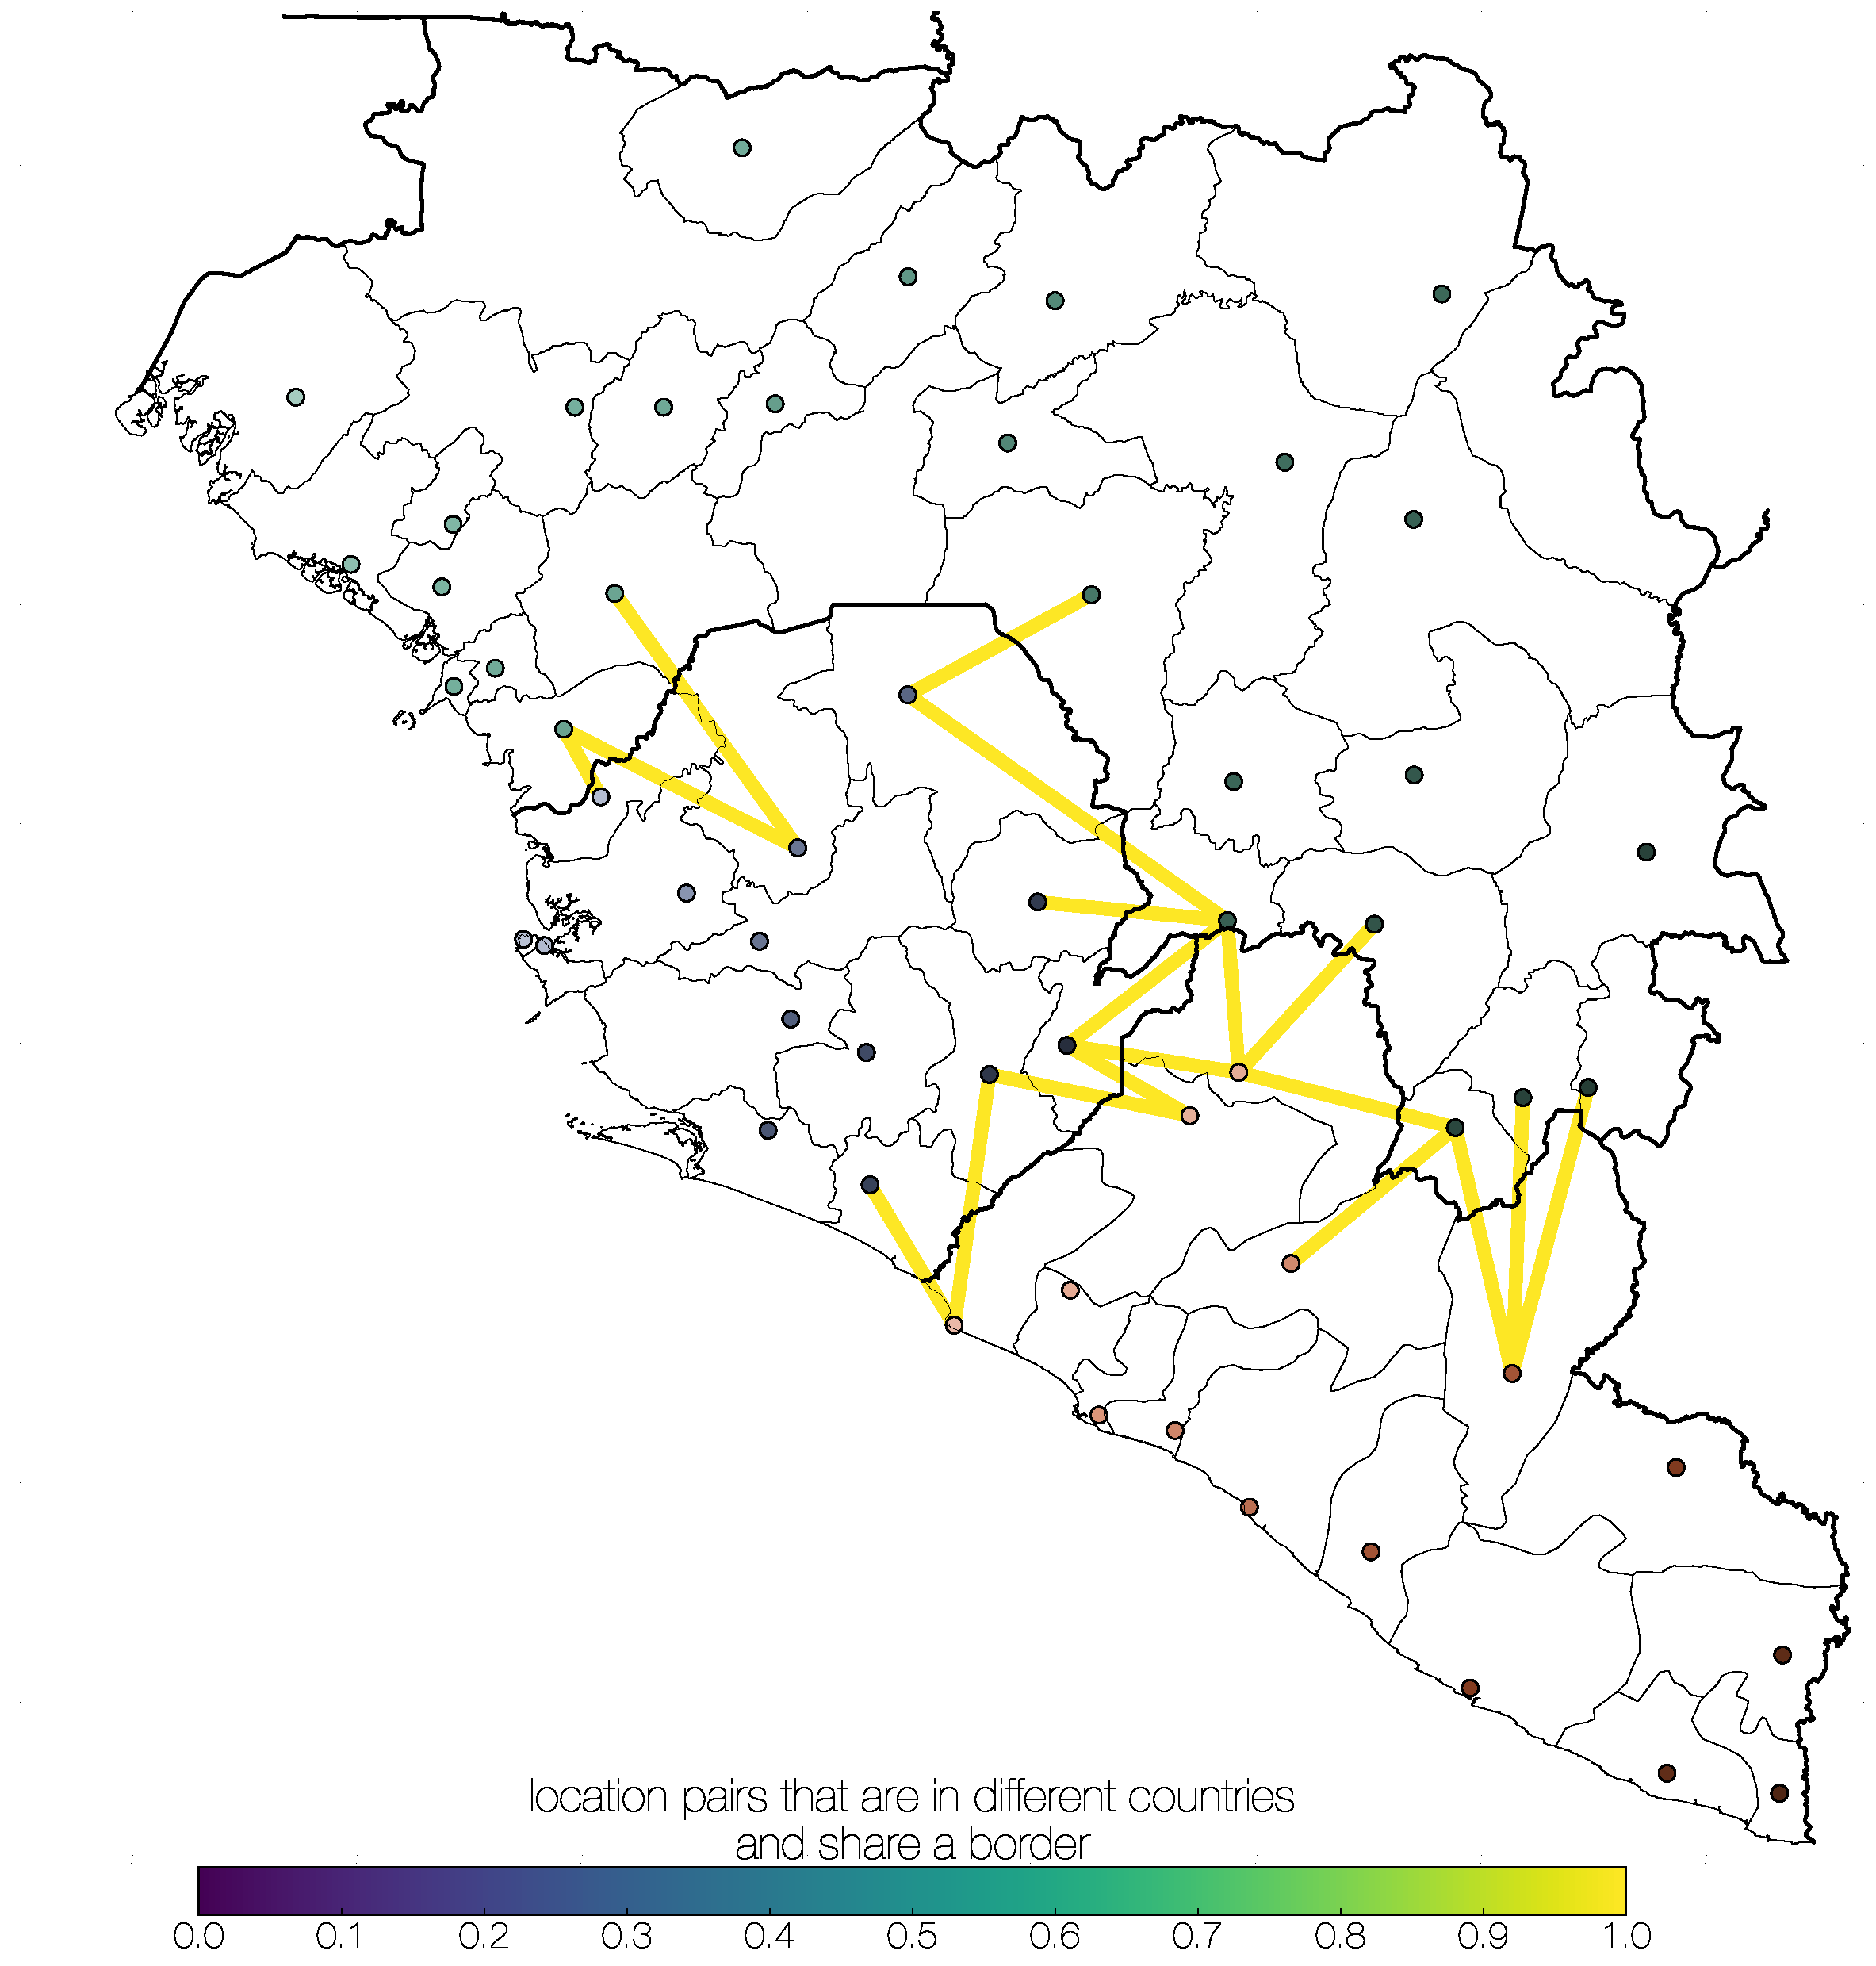
\includegraphics[width=50mm]{supp_figures/EBOV_predictorMap_international_border_shared.pdf} &   \includegraphics[width=65mm]{supp_figures/EBOV_predictor_withinCountry_heatmap.pdf} \\
	A) International border & B) Within country effect \\[6pt]
	 \includegraphics[width=50mm]{supp_figures/EBOV_predictorMap_destinationCaseCounts.pdf} &   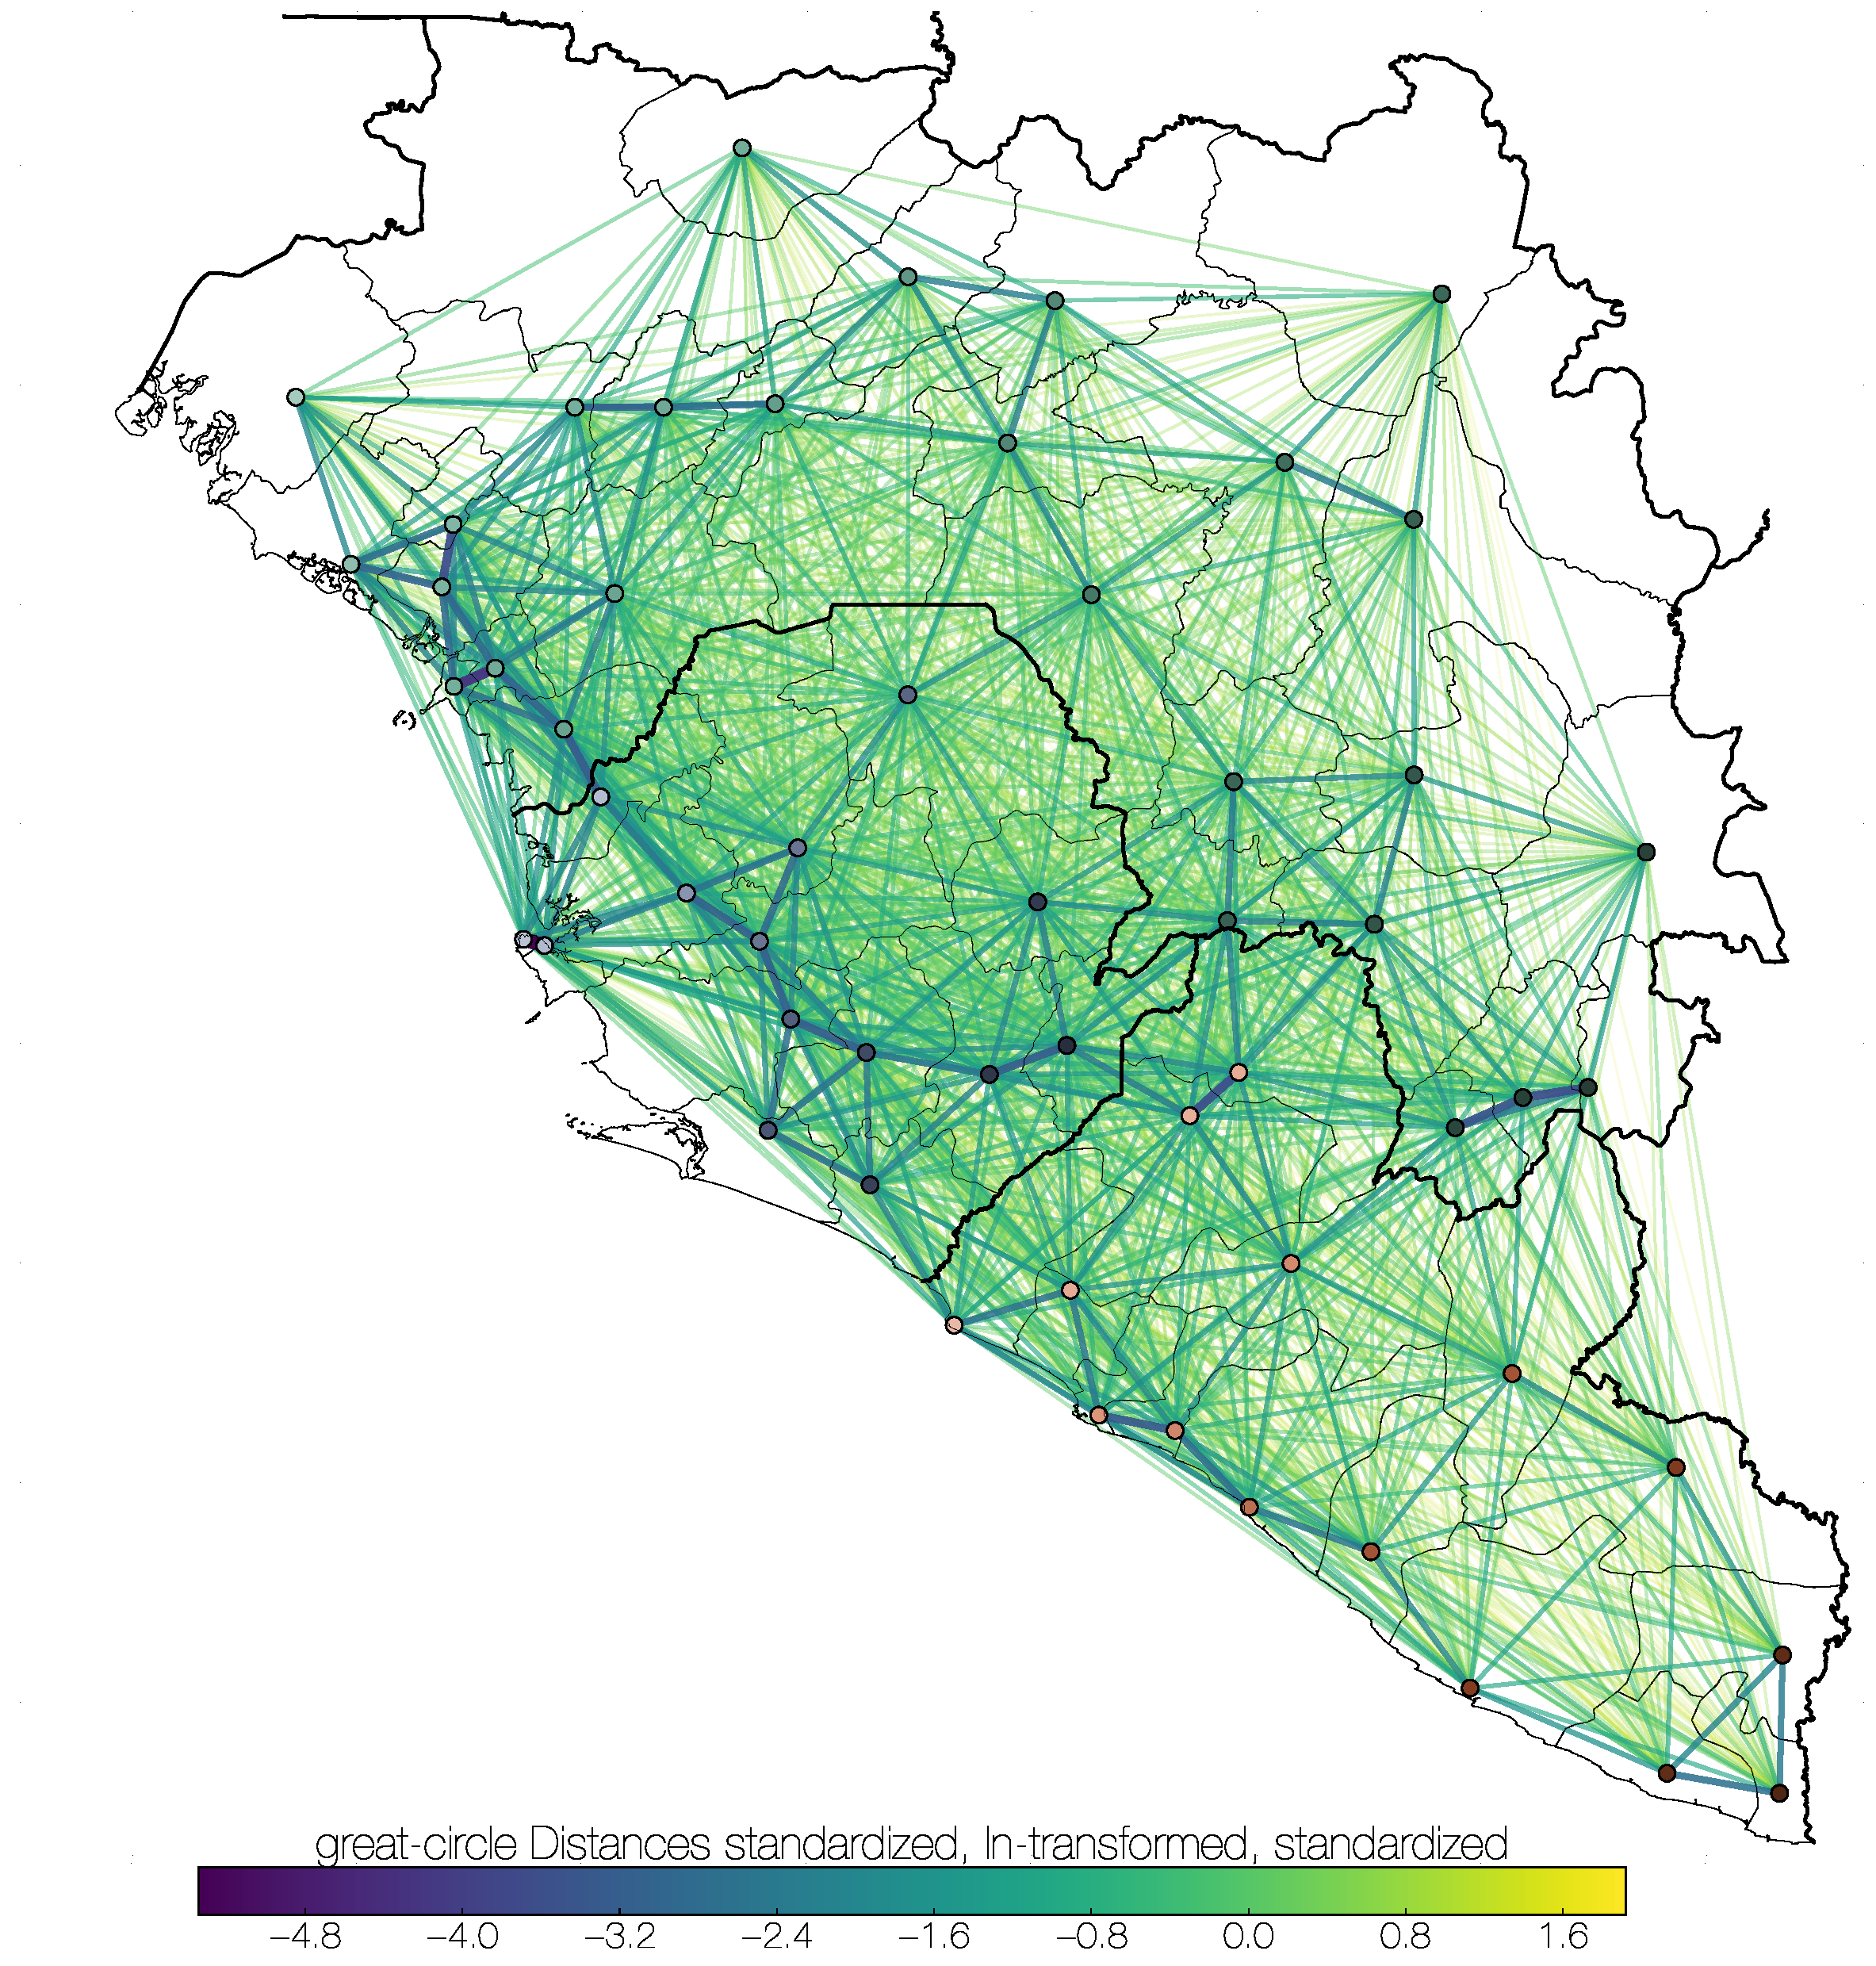
\includegraphics[width=50mm]{supp_figures/EBOV_predictorMap_greatCircleDistances.pdf} \\
	C) Location case counts & D) Great circle distances \\[6pt]
	\multicolumn{2}{c}{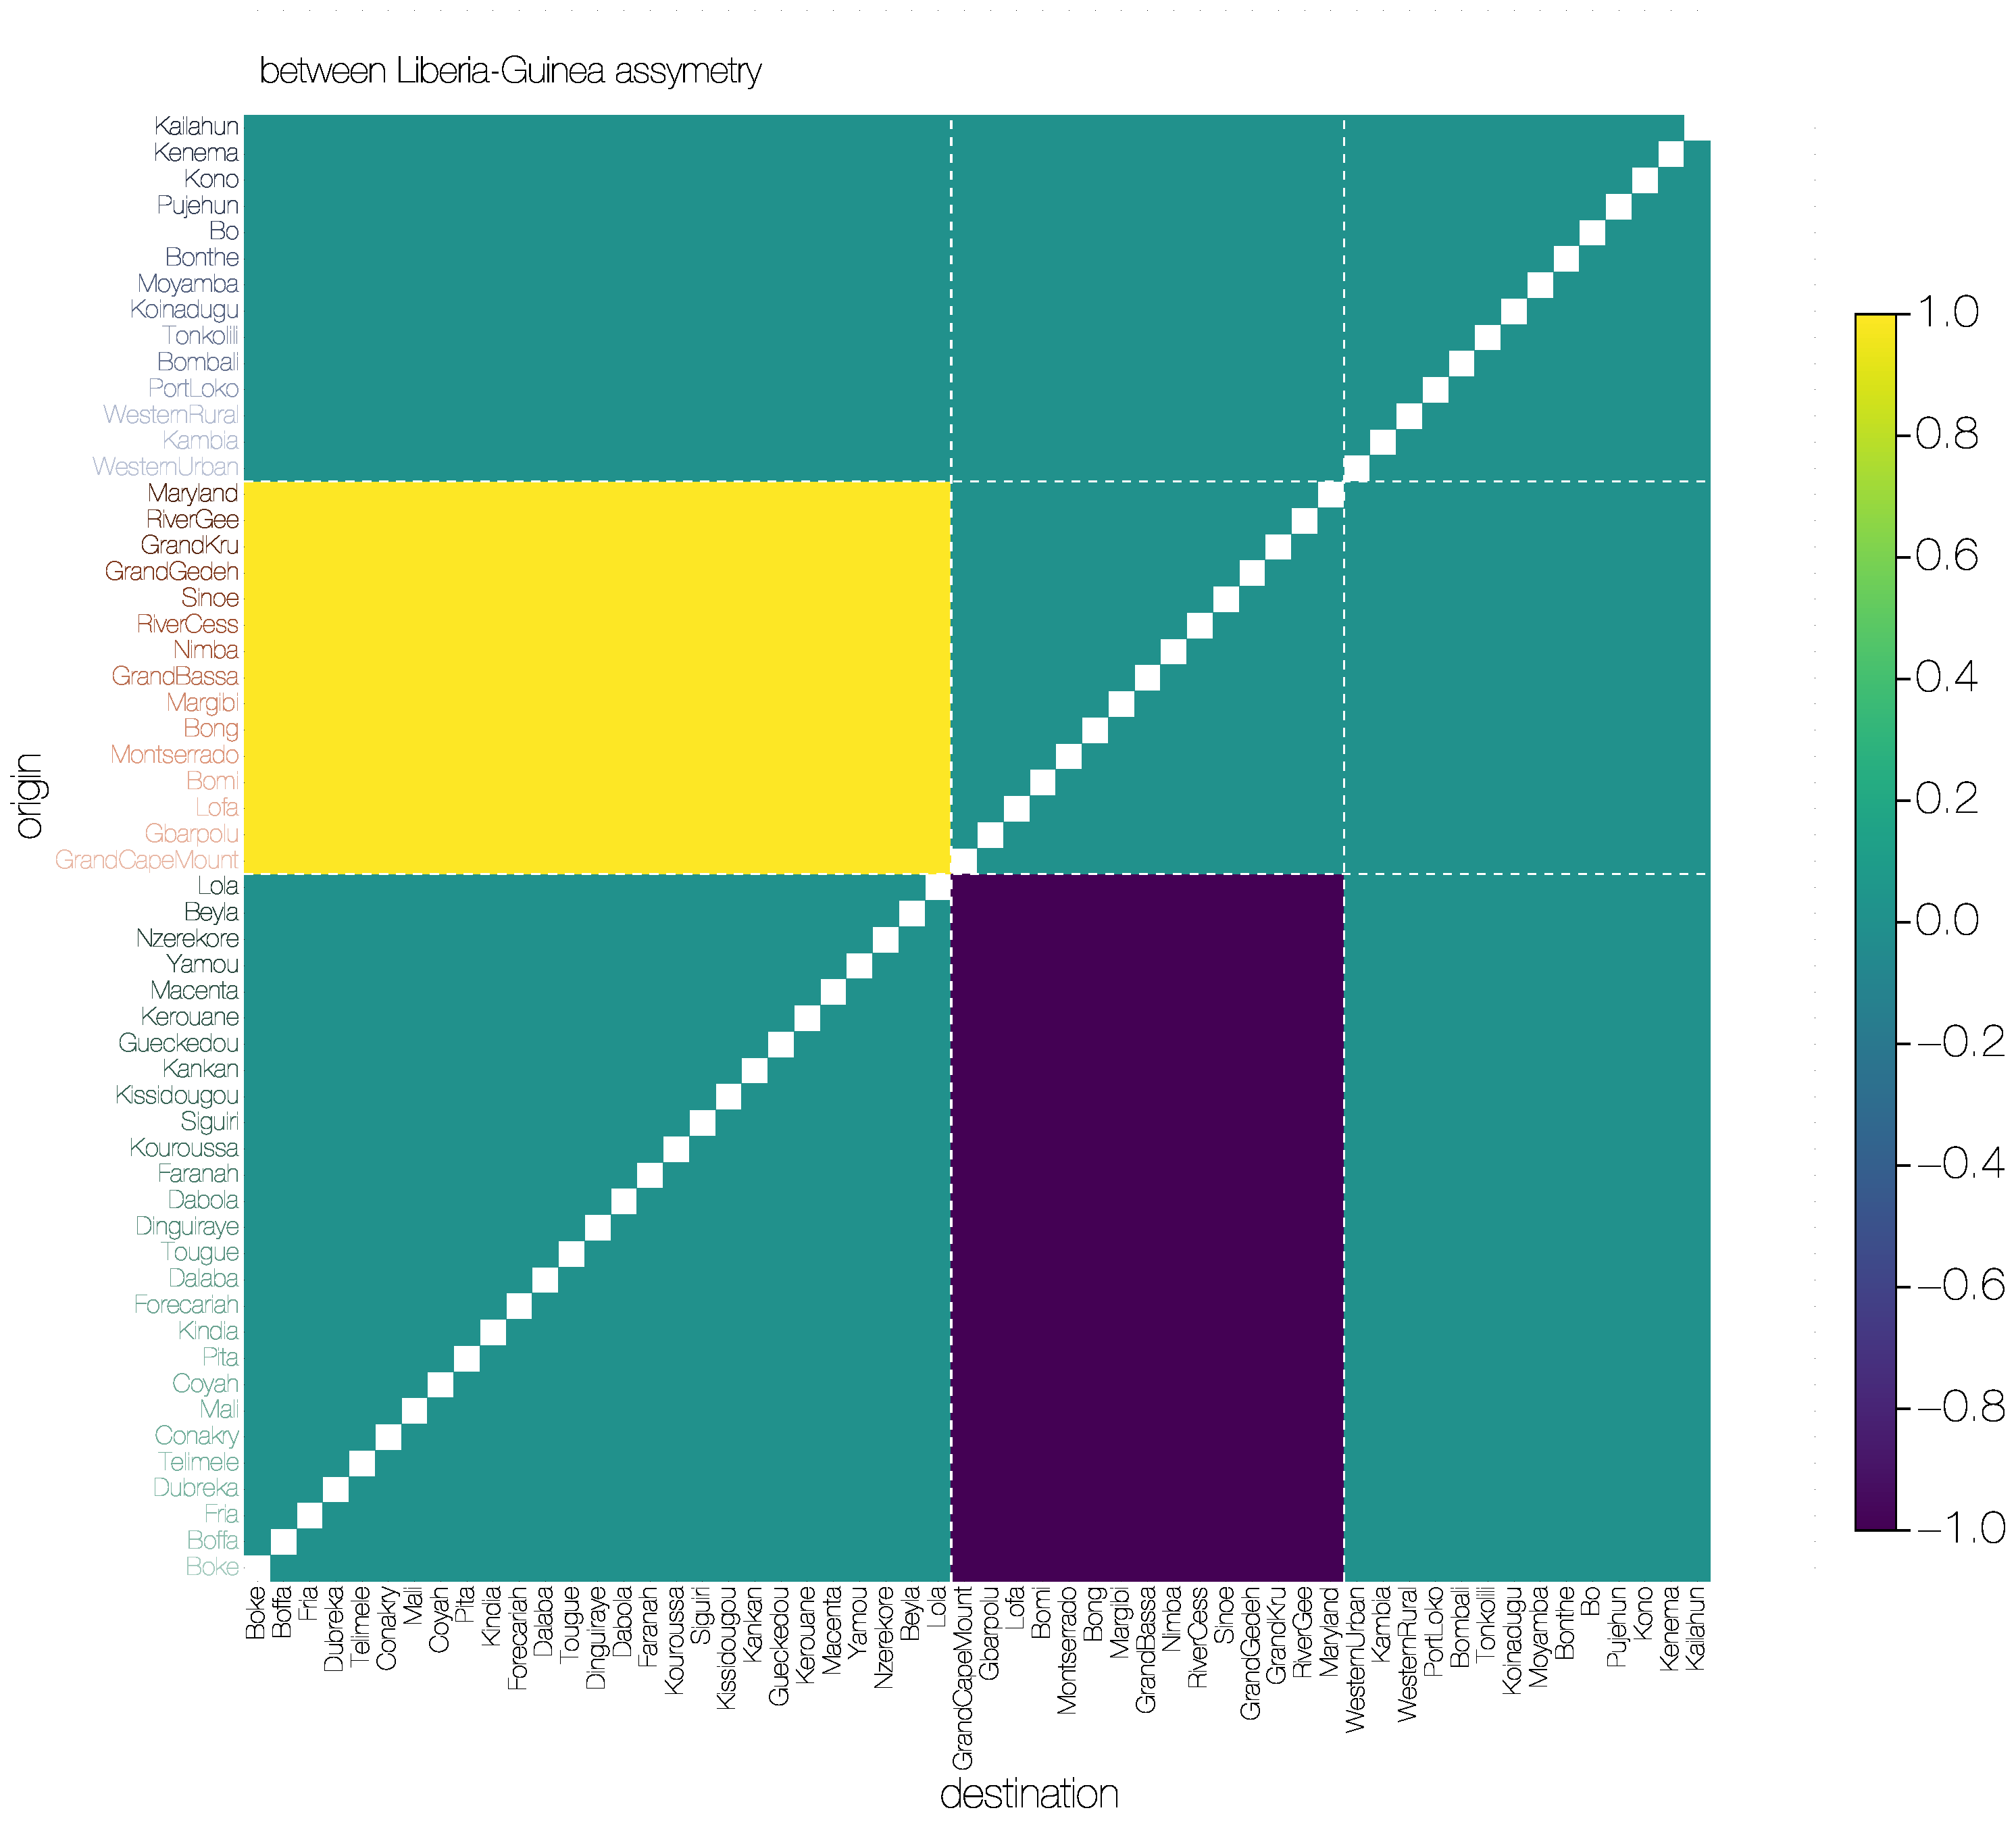
\includegraphics[width=65mm]{supp_figures/EBOV_predictor_betweenLBR_GIN_Assymetry_heatmap.pdf} }\\
	\multicolumn{2}{c}{E) Liberia-Guinea asymmetry}
	\end{tabular}
\caption{\textbf{Matrices of significant predictors.}
Six predictors were found to be strongly associated with Ebola virus migration between locations.
Visual representations of the matrices used are shown in A-E.
A) Connects location pairs that share an international border.
B) Shows the predictor matrix that was used to model within country effects.
C) Maps case counts at each location. This predictor has uniform values across rows or columns, for origin and destination predictor matrices, respectively.
D) Shows great circle distances between location population centroids.
E) Represents the predictor matrix for the Liberia-Guinea asymmetry effect.}
\label{predictor_maps}
\end{figure}

\begin{figure}[H]
 \centering		
	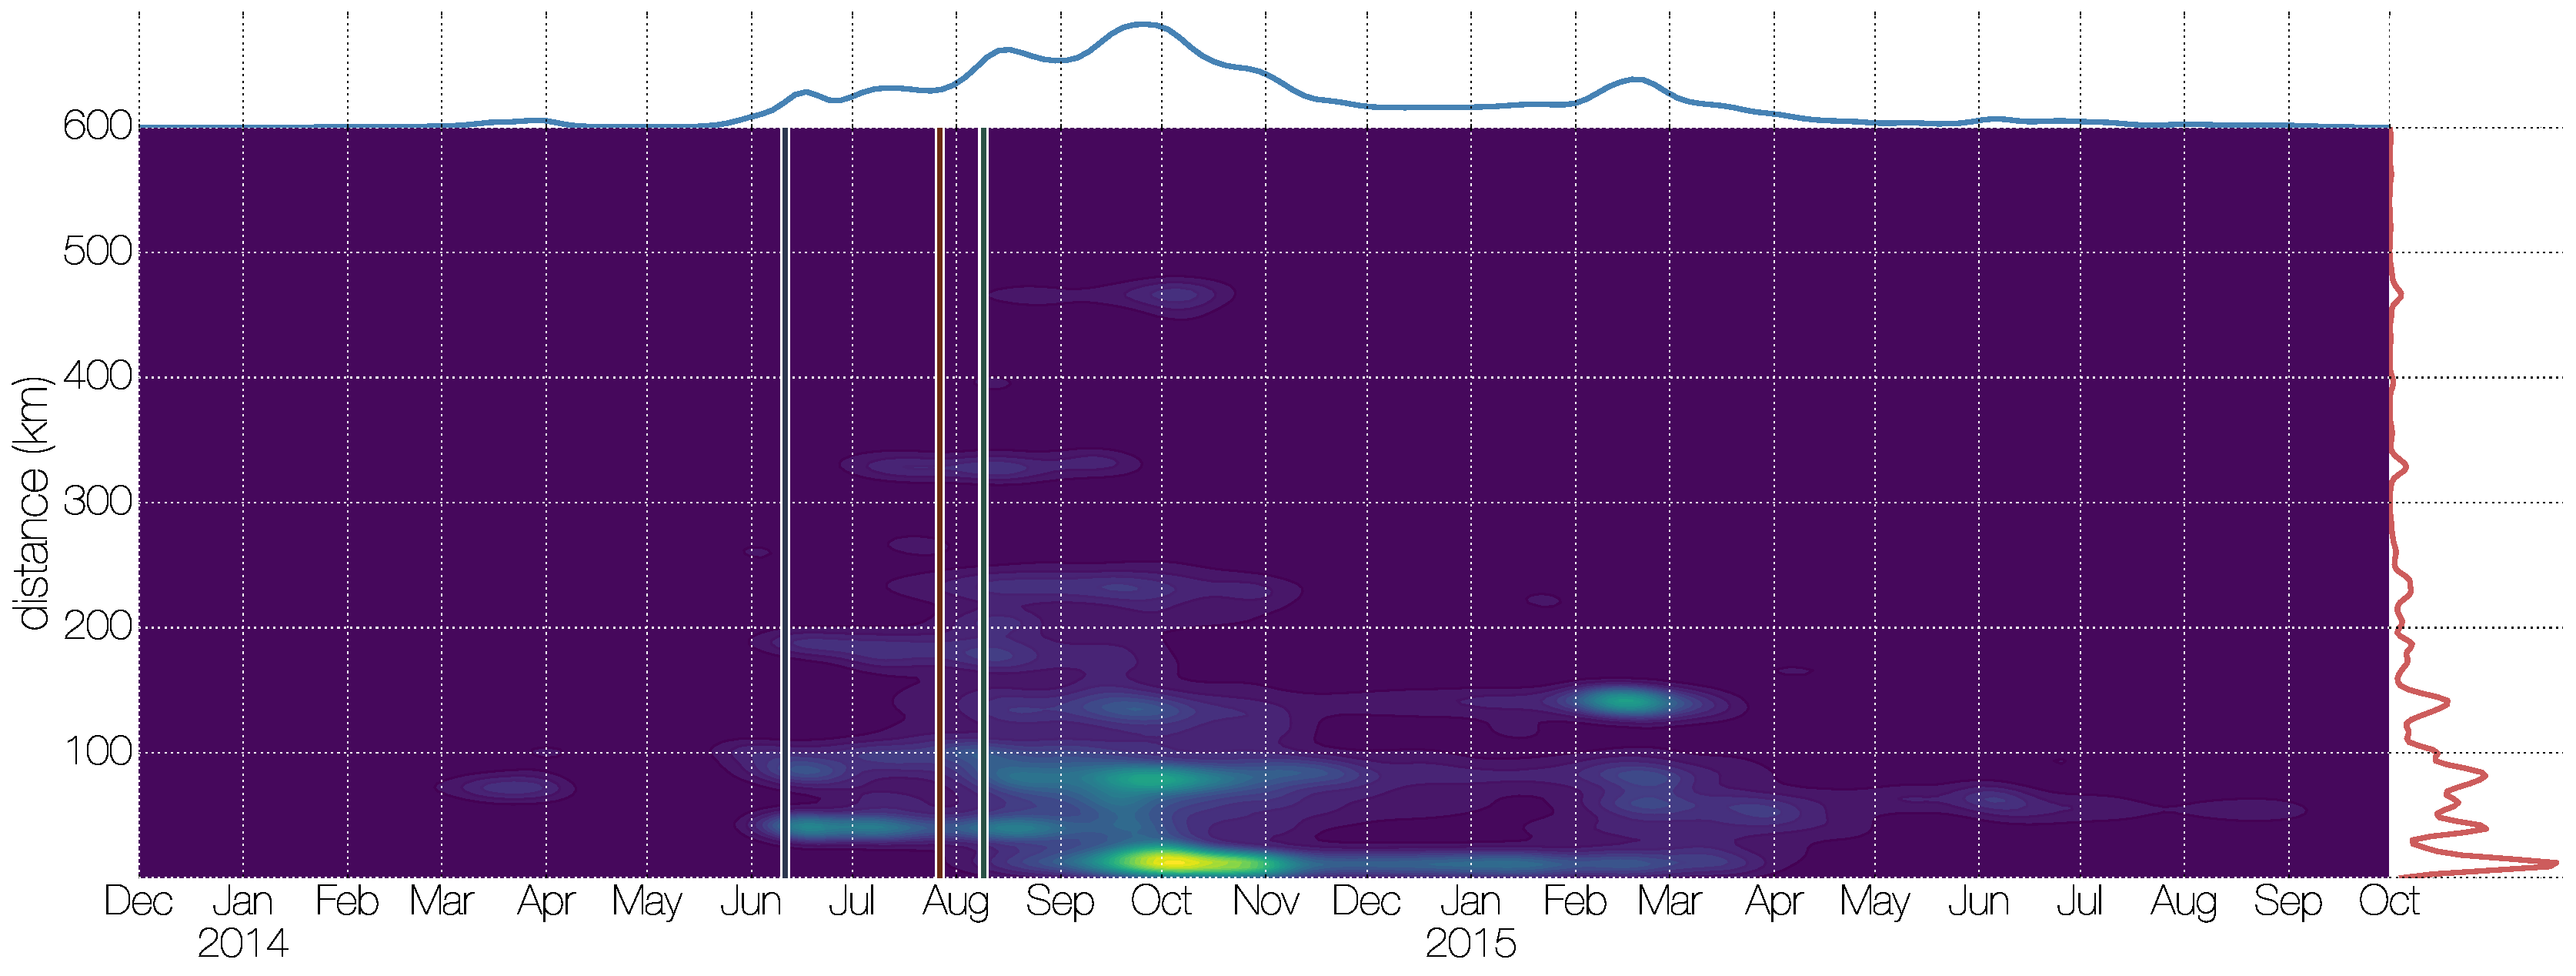
\includegraphics[width=0.85\textwidth]{supp_figures/EBOV_KDE2d_all.pdf}
	\caption{\textbf{Posterior density of location transitions over distance and time.}
	Contour plot showing the posterior density of location transitions over time (x axis) and distances (y axis).
	Lines at the top and to the right of the plot are 1 dimensional kernel density estimates of jump times (blue, top) and jump distances (red, right).
	Vertical lines indicate the dates of declared border closures by each of the tree countries: 11 June 2014 in Sierra Leone (blue), 27 July 2014 Liberia (red), and 09 August 2014 (green).
	}
	\label{all_jumps}
\end{figure}

\begin{figure}[H]
 \centering		
	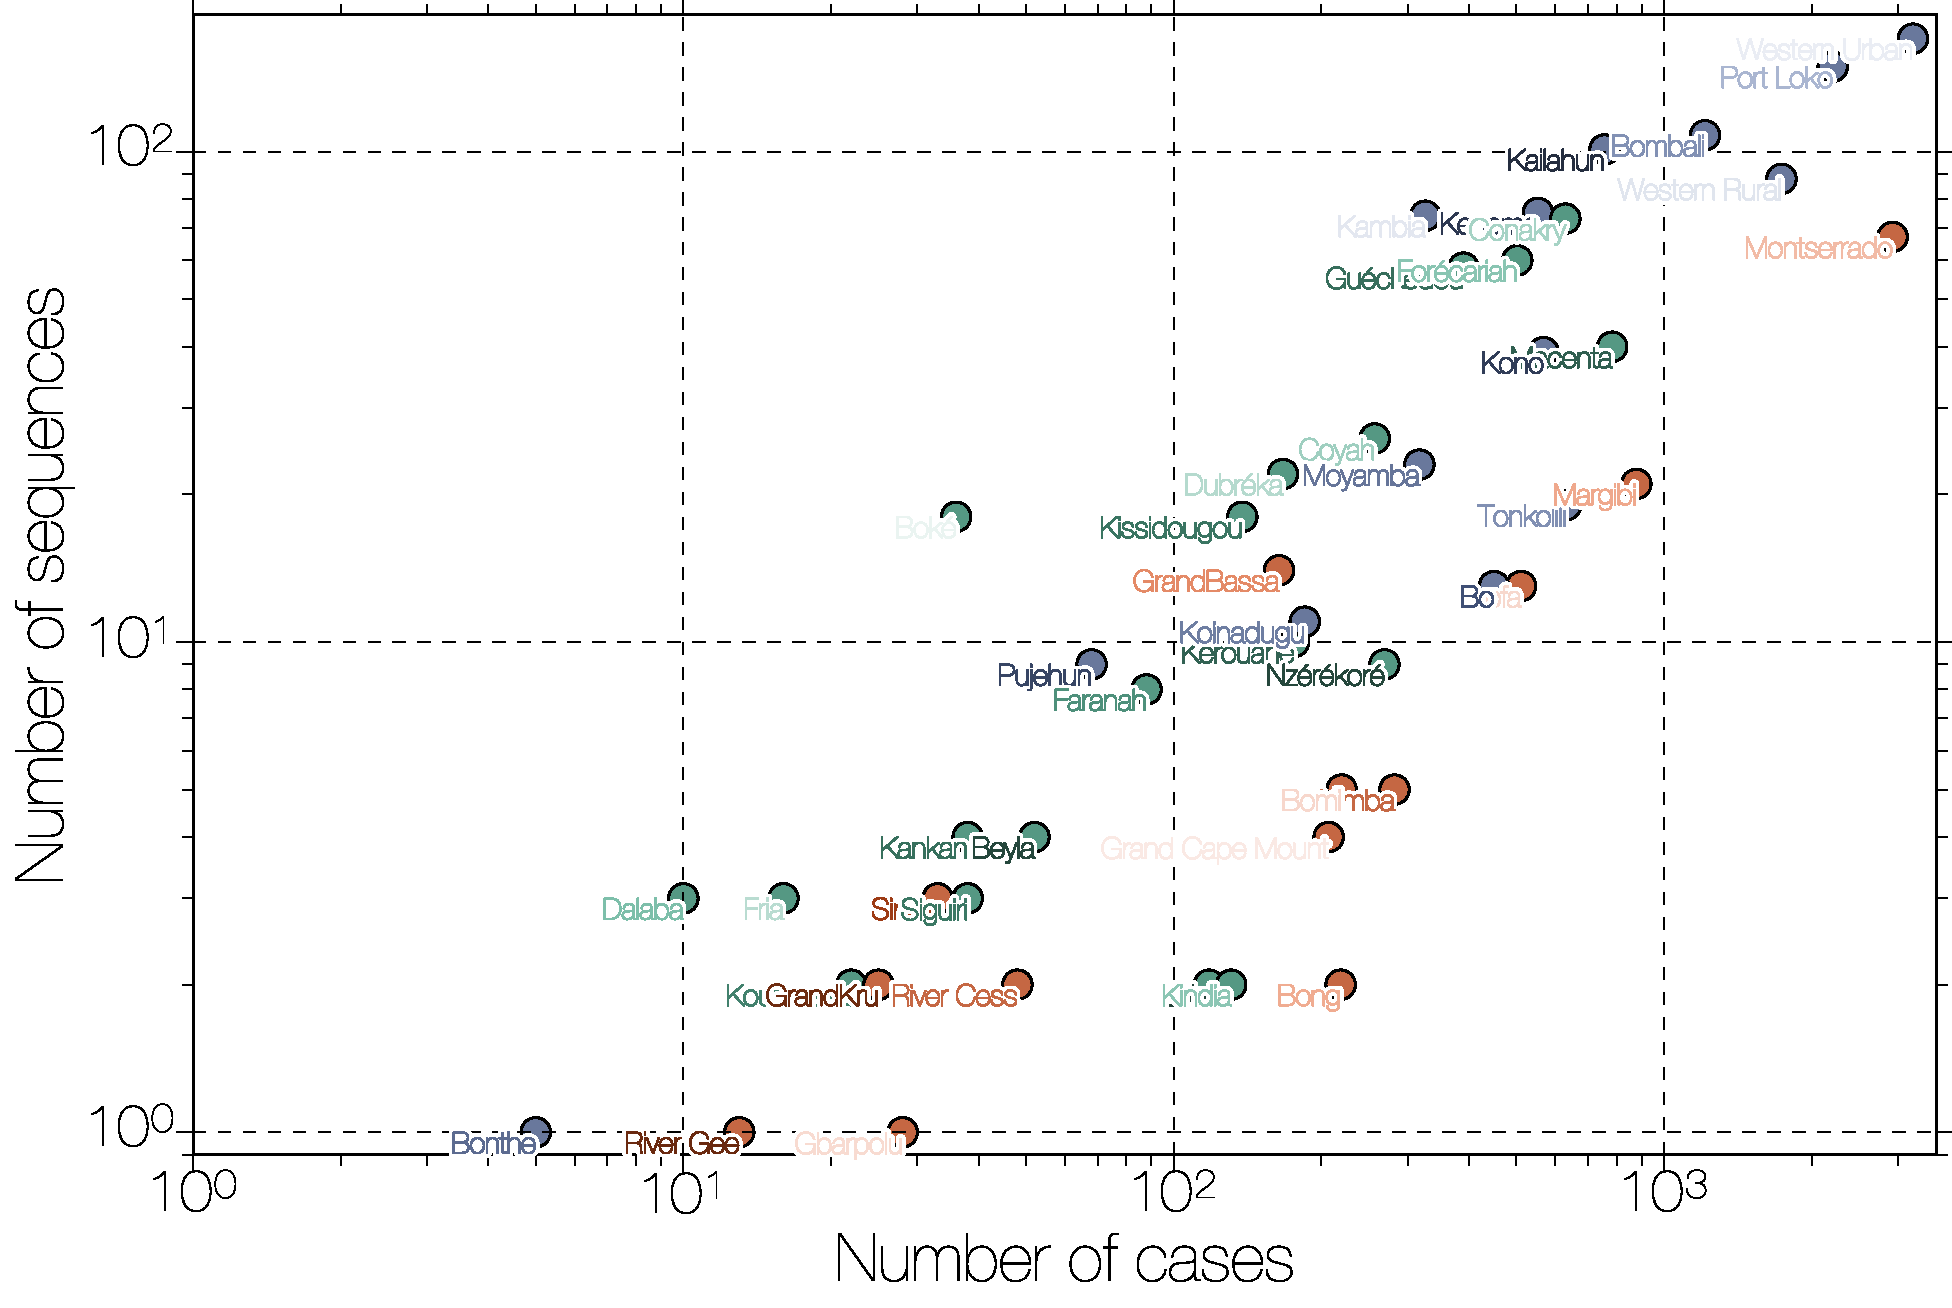
\includegraphics[width=0.85\textwidth]{supp_figures/EBOV_samplingCorrelations.pdf}
	\caption{\textbf{Correlation between number of cases and number of sequences for each location.}
	There is a strong relationship (Spearman correlation coefficient $=0.91$) between the number of sequences and the number of confirmed and suspected cases each location has.
	This indicates that despite large differences in case numbers between locations, the sampling of sequences has been scaled appropriately.
	}
	\label{sampling_correlation}
\end{figure}

\bibliographystyle{plainnat}
\bibliography{EBOV_phylogeography}

\end{document}
